% !TEX root = mythesis.tex

%==============================================================================
\chapter{Symmetries}
\label{sec:symmetries}
%==============================================================================

A very important aspect of the analysis are the symmetries. They let us extract useful information from the available data. We can leverage the symmetries we have found, so that we can reduce the numerical uncertainties of our data by averaging, or we can reduce the computational cost by declaring two results are the same by symmetry~\cite{evan}.

In this chapter we will see what is the symmetry of the lattice, which transformations are symmetry operators of the Hubbard model Hamiltonian, and how they transform the correlation functions that we are interested in. This will help us improve our data and the results we extract from it.

\section{Lattice}
\label{sec:lattice}
% Hexagonal lattice (BESTAGONAL :D)

The honeycomb lattice is a 2D lattice where the points of the primitive cell lie on the vertices of a hexagon. The reciprocal lattice is also hexagonal. The honeycomb lattice can be seen as made of two triangular lattices. Lattices with this property are called a bipartite. In general, a bipartite is any lattice which we can make from two overlapping lattices, where every point of one of the sublattices is only neighboring points from the other sublattice~\cite{graphhmc}. One of the triangular sublattices of the honeycomb plane is generated by two non-orthogonal vectors
\begin{equation}
  \vec{a}_1 = \frac{\sqrt{3}}{2}
  \begin{pmatrix}
    \sqrt{3} \\
    +1
  \end{pmatrix}, \qquad \qquad
  \vec{a}_2 = \frac{\sqrt{3}}{2}
  \begin{pmatrix}
    \sqrt{3} \\
    -1
  \end{pmatrix}.
\end{equation}
By repeating them $L_1$ and $L_2$ times respectively, we can construct the whole finite sublattice. The other one can be constructed simply by offsetting the points with a translation vector $\vec{r} = \pm(\vec{a}_1 + \vec{a}_2)$. On \cref{fig:bipartite} is shown the bipartite of the hexagonal lattice.
\begin{figure}
  \begin{center}
    \begin{tikzpicture}
      \foreach \j in {0,1}{
          \foreach \i in {0,1,2,3,4,5,6}{
              \def\spacing{1}
              % the integer division is an implicit floor
              \def\xshift{ \spacing*\i*(3/2) }
              \ifthenelse{\isodd{\i}}{
                  % in plane hexagons
                  \def\yshift{ sqrt(3)*(\j+0.5)*\spacing }
              } {
                  % higher hexagons
                  \def\yshift{ sqrt(3)*\j*\spacing }
              }
              
              \coordinate (A) at ({\xshift+\spacing}         ,{\yshift}                  );
              \coordinate (B) at ({\xshift+\spacing*cos(60)} ,{\yshift+\spacing*sin(60)} );
              \coordinate (C) at ({\xshift+\spacing*cos(120)},{\yshift+\spacing*sin(120)});
              \coordinate (D) at ({\xshift-\spacing}         ,{\yshift}                  );
              \coordinate (E) at ({\xshift+\spacing*cos(240)},{\yshift+\spacing*sin(240)});
              \coordinate (F) at ({\xshift+\spacing*cos(300)},{\yshift+\spacing*sin(300)});

              \draw[thick,dashed,black] (A) -- (B);
              \draw[thick,,dashed,black] (B) -- (C);
              \draw[thick,dashed,black] (C) -- (D);
              \draw[thick,dashed,black] (D) -- (E);
              \draw[thick,dashed,black] (E) -- (F);
              \draw[thick,dashed,black] (F) -- (A);

              \newdimen\r
              \r=2pt
              % Dirac points
              \filldraw[red] (A) circle (\r) node[anchor=north] {};
              \filldraw[blue] (B) circle (\r) node[anchor=south] {};
              \filldraw[red] (C) circle (\r) node[anchor=north] {};
              \filldraw[blue] (D) circle (\r) node[anchor=south] {};
              \filldraw[red] (E) circle (\r) node[anchor=north] {};
              \filldraw[blue] (F) circle (\r) node[anchor=south] {};
          }
      }
    \end{tikzpicture}
    \caption{Honeycomb lattice is a bipartite lattice because we can separate and label the lattice points with different colors (in this example blue and red) in such a way that every point in blue color neighbors only points with red color.}
    \label{fig:bipartite}
  \end{center}
\end{figure}

% Write what the symmetries of the lattice are
In order to investigate the symmetry operators and how they transform the correlation functions, we work with the reciprocal lattice. The primitive cell of the reciprocal is called Brillouin zone (BZ). Some points on the lattice which are of special interest have labels that are used in the literature and in this thesis. These are the center of the first Brillouin zone called the Gamma point ($\Gamma$), the two points on the vertices of the BZ called the Dirac points ($K, K'$), and the three middle of the edges of the BZ points $M, M', M''$. They are all shown on \cref{fig:points}, as well as their neighbors. The graph shows that the first BZ exhibits all the symmetries of the lattice, since the plane wave with a specific mode outside the 1st BZ is exactly equal to a plane wave with a momentum inside the BZ. Therefore, we do not need to investigate beyond it. So, we consider only the first Brillouin zone in our calculations.
\begin{figure}
\begin{center}
  \begin{tikzpicture}
    \newdimen\R
    \R=1cm
    \foreach \x/\y in
      {
        0/0,
        1.732050808/0,
        0.8660254038/1.5,
        -0.8660254038/1.5,
        -1.732050808/0,
        -0.8660254038/-1.5,
        0.8660254038/-1.5
      }
      {
        \begin{scope}[xshift=\x\R, yshift=\y\R]
          \draw (90:\R) \foreach \theta in {150,210,270,330,390,450} { -- (\theta:\R)};
        \end{scope};
      }
    \newdimen\r
    \r=2pt

    % Gamma points
    \filldraw[black] (0,0) circle (\r) node[anchor=north] {$\Gamma$};
    \filldraw[black] (1.732050808\R,0) circle (\r) node[anchor=north] {$\Gamma$};
    \filldraw[black] (0.8660254038\R, 1.5\R) circle (\r) node[anchor=north] {$\Gamma$};

    % Dirac points
    \filldraw[ForestGreen] (-30:\R) circle (\r) node[anchor=north] {$K'$};
    \foreach \theta in {90,210}{\filldraw[ForestGreen] (\theta:\R) circle (\r) ;};
    \filldraw[ForestGreen] (30:2\R) circle (\r) node[anchor=north] {$K'$};

    \filldraw[OliveGreen] (30:\R) circle (\r) node[anchor=south] {$K$};
    \foreach \theta in {150,270}{\filldraw[OliveGreen] (\theta:\R) circle (\r) ;};
    \filldraw[OliveGreen] (-30:2\R) circle (\r) node[anchor=south] {$K$};

    % M points
    \filldraw[RoyalBlue] (0:0.8660254038\R) circle (\r) node[anchor=east] {};
    \filldraw[RoyalBlue] (180:0.8660254038\R) circle (\r) node[anchor=east] {$M$};
    \filldraw[Cerulean]  (60:0.8660254038\R) circle (\r) node[anchor=south west] {};
    \filldraw[Cerulean]  (240:0.8660254038\R) circle (\r) node[anchor=north east] {$M'$};
    \filldraw[Blue] (120:0.8660254038\R) circle (\r) node[anchor=south east] {$M''$};
    \filldraw[Blue] (300:0.8660254038\R) circle (\r) node[anchor=north] {};

  \end{tikzpicture}
  \qquad
  \begin{tikzpicture}
    \def\spacing{3} 
    \coordinate (A) at ({\spacing*cos(330)},{\spacing*sin(330)});
    \coordinate (B) at ({\spacing*cos(30)} ,{\spacing*sin(30)} );
    \coordinate (C) at ({\spacing*cos(90)},{\spacing*sin(90)});
    \coordinate (D) at ({\spacing*cos(150)},{\spacing*sin(150)});
    \coordinate (E) at ({\spacing*cos(210)},{\spacing*sin(210)});
    \coordinate (F) at ({\spacing*cos(270)},{\spacing*sin(270)});

    \draw[thick,blue] (A) -- (B);
    \draw[thick,blue] (B) -- (C);
    \draw[thick,blue] (C) -- (D);
    \draw[thick,blue] (D) -- (E);
    \draw[thick,blue] (E) -- (F);
    \draw[thick,blue] (F) -- (A);

    \newdimen\r
    \r=2pt

    % Gamma points
    \filldraw[black] (0,0) circle (\r) node[anchor=north] {$\Gamma$};

    % Dirac points
    \filldraw[ForestGreen] (A) circle (\r) node[anchor=north] {$K'$};
    
    \filldraw[OliveGreen] (B) circle (\r) node[anchor=south] {$K$};

    % M points
    \filldraw[RoyalBlue] (0:0.8660254038*\spacing) circle (\r) node[anchor=east] {$M$};
    \filldraw[Cerulean]  (60:0.8660254038*\spacing) circle (\r) node[anchor=south west] {$M'$};
    \filldraw[Blue] (120:0.8660254038*\spacing) circle (\r) node[anchor=south east] {$M''$};

  \end{tikzpicture}
  \caption{LEFT: All points of special interest shown on the lattice and how they are copied over to other lattice cells. RIGHT: Special points only in the first BZ since it has all the symmetries of the lattice}
  \label{fig:points}
\end{center}
\end{figure}
% Group theory (dihhedral group, little group)
% Average points of the same symmetry operation 
The primitive cell of the reciprocal lattice of the honeycomb is a hexagon, meaning it must have all the symmetries of the dihedral group. The result is that each set of momenta that is related by symmetry of the lattice can be averaged (e.g., $K$ with $K'$, $M$ with $M'$ and $M''$, etc.). The key moment here is that we have not used any model here. This is only due to the symmetry of the lattice itself. Therefore, this averaging of momenta could be performed anytime, but the group symmetry operations are lattice dependent (Square, Honeycomb, Kagome, and others).

\section{Symmetry Operators}
\label{sec:sym-oper}
In this section, we are going to focus only on transformation that do not change the Hamiltonian in general or at half filling ($\mu=0$), i.e., symmetry operations which means they commute with it 
\begin{equation}
  [H,R] = 0.
\end{equation}
We can show that the expectation value of the operator does not change when we apply the symmetry to it.
\begin{equation}
 \langle \mathcal{O} \rangle = \frac{1}{Z} tr[\mathcal{O}R^{-1}Re^{-\beta H}] = \frac{1}{Z} tr[\mathcal{O}R^{-1}e^{-\beta H}R] = \frac{1}{Z} tr[R\mathcal{O}R^{-1}e^{-\beta H}] = \langle R\mathcal{O}R^{-1} \rangle.
\end{equation}
For our chosen model, there are only a few symmetry operators that satisfy this condition. We are going to see how they can be used to our advantage to increase our statistics~\cite{evan}.

% GIVE VISUAL EXAMPLES OF WHAT THE SYMMETRIES DO
\subsection{Spin-flip transformation}

On a bipartite lattice, we have a spin-flip operation that exchanges the particles and holes but leaves the charge untouched. On \cref{fig:spin-flip} there is shown an example of how the spin-flip operation transforms each operator when applied. Unfortunately, the example can show only how the spin and the charge transform, but not the Hamiltonian terms and amplitudes.
\begin{figure}
  \begin{center}
    \newcommand{\spinup}[2]{
    \draw[-Triangle , draw=#1, very thick] ([yshift=-1em]#2) -- ([yshift=1em]#2);
    }
    \newcommand{\spindown}[2]{
    \draw[Triangle- , draw=#1, very thick] ([yshift=-1em]#2) -- ([yshift=1em]#2);
    }
    \begin{tikzpicture}
      \tikzstyle{arrow} = [very thick,<->,>=stealth]
      \begin{scope}
        \def\spacing{3} 
        \coordinate (A) at ({\spacing}         ,{0}                  );
        \coordinate (B) at ({\spacing*cos(60)} ,{\spacing*sin(60)} );
        \coordinate (C) at ({\spacing*cos(120)},{\spacing*sin(120)});
        \coordinate (D) at ({-\spacing}         ,{0}                  );
        \coordinate (E) at ({\spacing*cos(240)},{\spacing*sin(240)});
        \coordinate (F) at ({\spacing*cos(300)},{\spacing*sin(300)});

        \draw[thin,dashed,black] (A) -- (B);
        \draw[thin,dashed,black] (B) -- (C);
        \draw[thin,dashed,black] (C) -- (D);
        \draw[thin,dashed,black] (D) -- (E);
        \draw[thin,dashed,black] (E) -- (F);
        \draw[thin,dashed,black] (F) -- (A);
        
        \spinup{blue}{A};
        \spinup{red}{B};
        \spindown{red}{C};
        \spinup{blue}{D};
        \spindown{blue}{E};
        \spindown{red}{F};
      \end{scope}

      \begin{scope}[xshift=9.5cm]
        \def\spacing{3} 
        \coordinate (A) at ({\spacing}         ,{0}                  );
        \coordinate (B) at ({\spacing*cos(60)} ,{\spacing*sin(60)} );
        \coordinate (C) at ({\spacing*cos(120)},{\spacing*sin(120)});
        \coordinate (D) at ({-\spacing}         ,{0}                  );
        \coordinate (E) at ({\spacing*cos(240)},{\spacing*sin(240)});
        \coordinate (F) at ({\spacing*cos(300)},{\spacing*sin(300)});
  
        \draw[thin,dashed,black] (A) -- (B);
        \draw[thin,dashed,black] (B) -- (C);
        \draw[thin,dashed,black] (C) -- (D);
        \draw[thin,dashed,black] (D) -- (E);
        \draw[thin,dashed,black] (E) -- (F);
        \draw[thin,dashed,black] (F) -- (A);
        
        \spindown{blue}{A};
        \spindown{red}{B};
        \spinup{red}{C};
        \spindown{blue}{D};
        \spinup{blue}{E};
        \spinup{red}{F};
      \end{scope}

      \draw[arrow] (3.5,0) -- (6,0) node [midway, sloped, above] {$I$};
    \end{tikzpicture}    
  \end{center}
  \caption{An example of the spin-flip transformation with all possibilities of creation/annihilation operators. The graphs show only the transformation of the charge and the spin of the operators. The color of the arrows shows the charge (blue = $+1$, red = $-1$) and the orientation shows the spin. We can go back and forth between the left and the right graphs by using the spin-flip conjugation.}
  \label{fig:spin-flip}
\end{figure}

When applied onto the creation/annihilation operators of the particles and the holes, this spin transformation gives us

\begin{equation}
  \begin{aligned}
    IpI^{-1} &= \Sigma h^\dagger = h^\dagger \Sigma, & IhI^{-1} &= \Sigma p^\dagger = p^\dagger \Sigma, \\
    Ip^\dagger I^{-1} &= \Sigma h = h \Sigma, & Ih^\dagger I^{-1} &= \Sigma p = p \Sigma,
  \end{aligned}
\end{equation}
where $\Sigma$ is a matrix which shows us the behavior of the bipartite lattice
\begin{equation}
  \Sigma_{xy} = (-1)^x\delta_{xy}.
\end{equation}
We can check if this symmetry commutes with the Hamiltonian by first showing that it leaves the charge invariant
\begin{equation}
  IqI^{-1} = Ip^\dagger I^{-1}IpI^{-1} - Ih^\dagger I^{-1}IhI^{-1} = h\Sigma\Sigma h^\dagger - p\Sigma\Sigma p^\dagger = (1 - h^\dagger h) - (1 - p^\dagger p) = p^\dagger p - h^\dagger h = q.
  \label{eq:spin-charge}
\end{equation}
It can also be shown that the third component of the spin gets flipped after we apply this operator
\begin{equation}
  Is^3I^{-1} = -s^3,
\end{equation}
where
\begin{equation}
  s^3_x = \frac{1}{2}\left(\delta_{xx} - p^\dagger_x p_x - h^\dagger_x h_x\right)
\end{equation}
Finally, it is important to see how the hopping term transforms under this symmetry operation
\begin{equation}
  \begin{aligned}
    I\left( -\sum_{xy} p^\dagger_x K_{xy} p_y + \sigma_k h^\dagger_x K_{xy} h_y\right) I^{-1} &= -\sum_{xy} I p^\dagger_x I^{-1}I K_{xy} I^{-1}I p_y I^{-1} + \sigma_k I h^\dagger_x I^{-1}I K_{xy} I^{-1}I h_y I^{-1}
    \\
    &= -\sum_{xy}  h_x (\Sigma I K I^{-1}\Sigma)_{xy} h^\dagger_y + \sigma_k p_x (\Sigma I K I^{-1}\Sigma)_{xy} p^\dagger_y
    \\
    &= -\sum_{xy} -(\delta_{xy} (I K I^{-1})_{xy} - h^\dagger_y (I K I^{-1})_{xy} h_x) -
    \\
    &- \sigma_k (\delta_{xy} (I K I^{-1})_{xy} - p^\dagger_y (I K I^{-1})_{xy} p_x)
    \\
    &= \sigma_k \left[-\sum_{xy} p^\dagger_x (I K I^{-1})^\top_{xy} p_y + \sigma_k h^\dagger_x (I K I^{-1})^\top_{xy} h_y \right],
  \end{aligned}
\end{equation}
in which $\Sigma K \Sigma = -K$, $tr[K] = 0$, and $\sigma^2_k = 1$. In general, to return to our initial hopping term, we need $I$ to be anti-unitary where $IKI^{-1} = K^*$, and then we could replace $K^\dagger\rightarrow K$. Since we are working on a bipartite lattice, $K$ is a real valued matrix, resulting in $IKI^{-1} = K$ and $K^\dagger = K^* = K^\top = K$; we can choose $\sigma_k = 1$ because of the Honeycomb, which even for $\mu \neq 0$ gives us the commutator $[H - \vec{\mu}\cdot\vec{q}, I] = 0$. This is true because as shown in \cref{eq:spin-charge} the charge is even in relation to the spin-flip symmetry operation.

\subsection{Charge transformation}

Another symmetry we can consider is the charge symmetry operation. It exchanges the charges but leaves the spin fixed. When applied onto the creation and annihilation operators, it transforms them as 
\begin{equation}
  \begin{aligned}
    CpC^{-1} &= h, & ChC^{-1} &= p, \\
    Cp^\dagger C^{-1} &= h^\dagger, & Ch^\dagger C^{-1} &= p^\dagger.
  \end{aligned}
\end{equation}
On \cref{fig:charge-flip} is shown how the charge and spin of all creation/annihilation operators transform under this symmetry operation.
\begin{figure}
  \begin{center}
    \newcommand{\spinup}[2]{
    \draw[-Triangle , draw=#1, very thick] ([yshift=-1em]#2) -- ([yshift=1em]#2);
    }
    \newcommand{\spindown}[2]{
    \draw[Triangle- , draw=#1, very thick] ([yshift=-1em]#2) -- ([yshift=1em]#2);
    }
    \begin{tikzpicture}
      \tikzstyle{arrow} = [very thick,<->,>=stealth]
      \begin{scope}
        \def\spacing{3} 
        \coordinate (A) at ({\spacing}         ,{0}                  );
        \coordinate (B) at ({\spacing*cos(60)} ,{\spacing*sin(60)} );
        \coordinate (C) at ({\spacing*cos(120)},{\spacing*sin(120)});
        \coordinate (D) at ({-\spacing}         ,{0}                  );
        \coordinate (E) at ({\spacing*cos(240)},{\spacing*sin(240)});
        \coordinate (F) at ({\spacing*cos(300)},{\spacing*sin(300)});

        \draw[thin,dashed,black] (A) -- (B);
        \draw[thin,dashed,black] (B) -- (C);
        \draw[thin,dashed,black] (C) -- (D);
        \draw[thin,dashed,black] (D) -- (E);
        \draw[thin,dashed,black] (E) -- (F);
        \draw[thin,dashed,black] (F) -- (A);
        
        \spinup{blue}{A};
        \spinup{red}{B};
        \spindown{red}{C};
        \spinup{blue}{D};
        \spindown{blue}{E};
        \spindown{red}{F};
      \end{scope}

      \begin{scope}[xshift=9.5cm]
        \def\spacing{3} 
        \coordinate (A) at ({\spacing}         ,{0}                  );
        \coordinate (B) at ({\spacing*cos(60)} ,{\spacing*sin(60)} );
        \coordinate (C) at ({\spacing*cos(120)},{\spacing*sin(120)});
        \coordinate (D) at ({-\spacing}         ,{0}                  );
        \coordinate (E) at ({\spacing*cos(240)},{\spacing*sin(240)});
        \coordinate (F) at ({\spacing*cos(300)},{\spacing*sin(300)});
  
        \draw[thin,dashed,black] (A) -- (B);
        \draw[thin,dashed,black] (B) -- (C);
        \draw[thin,dashed,black] (C) -- (D);
        \draw[thin,dashed,black] (D) -- (E);
        \draw[thin,dashed,black] (E) -- (F);
        \draw[thin,dashed,black] (F) -- (A);
        
        \spinup{red}{A};
        \spinup{blue}{B};
        \spindown{blue}{C};
        \spinup{red}{D};
        \spindown{red}{E};
        \spindown{blue}{F};
      \end{scope}

      \draw[arrow] (3.5,0) -- (6,0) node [midway, sloped, above] {$C$};
    \end{tikzpicture}
  \end{center}
  \caption{An example of the charge transformation with all possibilities of creation/annihilation operators. The graphs show only the transformation of the charge and the spin of the operators. The color of the arrows shows the charge (blue = $+1$, red = $-1$) and the orientation shows the spin. We can go back and forth between the left and the right graphs by using the charge-flip conjugation.}
  \label{fig:charge-flip}
\end{figure}
If we conjugate with the charge operator, we get
\begin{equation}
  CqC^{-1} = Cp^\dagger C^{-1}CpC^{-1} - Ch^\dagger C^{-1}ChC^{-1} = h^\dagger h - p^\dagger p = -q
  \label{eq:charge-charge}
\end{equation}
and when conjugated with the spin operator
\begin{equation}
  Cs^3C^{-1} = s^3,
\end{equation}
so the spin is fixed for this operation. Again, we want to calculate the conjugation of the tight-binding term in the Hamiltonian with the charge-flip operator

\begin{equation}
  \begin{aligned}
    C\left( -\sum_{xy} p^\dagger_x K_{xy} p_y + \sigma_k h^\dagger_x K_{xy} h_y\right) C^{-1} &= -\sum_{xy} C p^\dagger_x C^{-1}C K_{xy} C^{-1}C p_y C^{-1} + \sigma_k C h^\dagger_x C^{-1}C K_{xy} C^{-1}C h_y C^{-1}
    \\
    &= -\sum_{xy}  h^\dagger_x (C K C^{-1})_{xy} h_y + \sigma_k p^\dagger_x (C K C^{-1})_{xy} p_y
    \\
    &= -\sum_{xy}  \sigma_k p^\dagger_x (C K C^{-1})_{xy} p_y + h^\dagger_x (C K C^{-1})_{xy} h_y,
  \end{aligned}
\end{equation}
where if we choose $CKC^{-1} = K$, we get to the initial term. Therefore, we are shown that on a bipartite lattice where we can choose $\sigma_k = +1$, we have a charge conjugation symmetry i.e. it commutes with the tight-binding Hamiltonian $[H,C] = 0$. This is because as shown in (\cref{eq:charge-charge}) the charge operator is flipped, but the interaction is even under this transformation because it is of the form $qVq$.

\subsection{Particle-hole transformation}

The particle-hole symmetry operator is a combination of two symmetry operators that do not transform the Hamiltonian nicely, but their combination does. It preserves the energy of the system, but flips the charge and the spin. This means that we should only consider the tight-binding Hamiltonian, i.e. the Hamiltonian without the chemical potential term.

In order to convince ourselves of the neat transformation and also the commutation of the Hamiltonian with the symmetry operator, we should first see how the constituent operators transform the Hubbard model Hamiltonian.

First, we look at the staggering operator $X$. It transforms the creation/annihilation operators like
\begin{equation}
  \begin{aligned}
    Xp^\dagger X^{-1} &= \Sigma p^\dagger = p^\dagger \Sigma, & Xh^\dagger X^{-1} &= \Sigma h^\dagger = h^\dagger \Sigma, \\
    Xp X^{-1} &= \Sigma p = p \Sigma, & XhX^{-1} &= \Sigma h = h \Sigma.
  \end{aligned}
\end{equation}
It leaves the charge, spin, and number operators invariant, but it flips the sign of the hopping term

\begin{equation}
  \begin{aligned}
    X\left( -\sum_{xy} p^\dagger_x K_{xy} p_y + \sigma_k h^\dagger_x K_{xy} h_y\right) X^{-1} &= -\sum_{xy} X p^\dagger_x X^{-1}X K_{xy} X^{-1}X p_y X^{-1} + \sigma_k X h^\dagger_x X^{-1}X K_{xy} X^{-1}X h_y X^{-1}
    \\
    &= -\sum_{xy}  p^\dagger_x (\Sigma X K X^{-1}\Sigma)_{xy} p_y + \sigma_k h^\dagger_x (\Sigma X K X^{-1}\Sigma)_{xy} h_y
    \\
    &= -\sum_{xy}  p^\dagger_x (\Sigma K \Sigma)_{xy} p_y + \sigma_k h^\dagger_x (\Sigma K \Sigma)_{xy} h_y
    \\
    &= -\left[-\sum_{xy} p^\dagger_x K_{xy} p_y + \sigma_k h^\dagger_x K_{xy} h_y \right].
  \end{aligned}
\end{equation}

The other operator that we consider is the one that "flips" the dagger of the operators. It transforms the particle/hole operators as

\begin{equation}
  \begin{aligned}
    FpF^{-1} &= p^\dagger, & FhF^{-1} &= h^\dagger, \\
    Fp^\dagger F^{-1} &= p, & Fh^\dagger F^{-1} &= h.
  \end{aligned}
\end{equation}
When applied onto the charge operator, it flips the sign $q \rightarrow -q$ which is shown below

\begin{equation}
  FqF^{-1} = Fp^\dagger F^{-1}FpF^{-1} - Fh^\dagger F^{-1}FhF^{-1} = p p^\dagger - h h^\dagger = (1 - p^\dagger p) - (1 - h^\dagger h) = -q.
\end{equation}
This in turn means that this symmetry operation flips the chemical potential and more importantly the hopping term
\begin{equation}
  \resizebox{\hsize}{!}{
  $\begin{aligned}
    F\left( -\sum_{xy} p^\dagger_x K_{xy} p_y + \sigma_k h^\dagger_x K_{xy} h_y\right) F^{-1} &= -\sum_{xy} F p^\dagger_x F^{-1}F K_{xy} F^{-1}F p_y F^{-1} + \sigma_k F h^\dagger_x F^{-1}F K_{xy} F^{-1}F h_y F^{-1}
    \\
    &= -\sum_{xy}  p_x (F K F^{-1})_{xy} p^\dagger_y + \sigma_k h_x (F K F^{-1})_{xy} h^\dagger_y
    \\
    &= -\sum_{xy} (\delta_{xy} (F K F^{-1})_{xy} - p^\dagger_y (F K F^{-1})_{xy} p_x) + \sigma_k (\delta_{xy} (F K F^{-1})_{xy} - h^\dagger_y (F K F^{-1})_{xy} h_x)
    \\
    &= - \left[ - \sum_{xy} p^\dagger_y (F K F^{-1})_{xy} p_x + \sigma_k h^\dagger_y (F K F^{-1})_{xy} h_x \right]
    \\
    &= - \left[ - \sum_{xy} p^\dagger_x (F K F^{-1})^\top_{xy} p_y + \sigma_k h^\dagger_x (F K F^{-1})^\top_{xy} h_y \right]
  \end{aligned}$
  }
\end{equation}
where $tr[K] = 0$, if we want to return to the original hopping term then we have to choose $F K F^{-1} = K^*$, and then we can substitute $K^\dagger \rightarrow K$. We see on  \cref{fig:dagger-flip} an example of the dagger-flip operator switching the signs of the charge and the spin.
\begin{figure}
  \begin{center}
    \newcommand{\spinup}[2]{
    \draw[-Triangle , draw=#1, very thick] ([yshift=-1em]#2) -- ([yshift=1em]#2);
    }
    \newcommand{\spindown}[2]{
    \draw[Triangle- , draw=#1, very thick] ([yshift=-1em]#2) -- ([yshift=1em]#2);
    }
    \begin{tikzpicture}
      \tikzstyle{arrow} = [very thick,<->,>=stealth]
      \begin{scope}
        \def\spacing{3} 
        \coordinate (A) at ({\spacing}         ,{0}                  );
        \coordinate (B) at ({\spacing*cos(60)} ,{\spacing*sin(60)} );
        \coordinate (C) at ({\spacing*cos(120)},{\spacing*sin(120)});
        \coordinate (D) at ({-\spacing}         ,{0}                  );
        \coordinate (E) at ({\spacing*cos(240)},{\spacing*sin(240)});
        \coordinate (F) at ({\spacing*cos(300)},{\spacing*sin(300)});

        \draw[thin,dashed,black] (A) -- (B);
        \draw[thin,dashed,black] (B) -- (C);
        \draw[thin,dashed,black] (C) -- (D);
        \draw[thin,dashed,black] (D) -- (E);
        \draw[thin,dashed,black] (E) -- (F);
        \draw[thin,dashed,black] (F) -- (A);
        
        \spinup{blue}{A};
        \spinup{red}{B};
        \spindown{red}{C};
        \spinup{blue}{D};
        \spindown{blue}{E};
        \spindown{red}{F};
      \end{scope}

      \begin{scope}[xshift=9.5cm]
        \def\spacing{3} 
        \coordinate (A) at ({\spacing}         ,{0}                  );
        \coordinate (B) at ({\spacing*cos(60)} ,{\spacing*sin(60)} );
        \coordinate (C) at ({\spacing*cos(120)},{\spacing*sin(120)});
        \coordinate (D) at ({-\spacing}         ,{0}                  );
        \coordinate (E) at ({\spacing*cos(240)},{\spacing*sin(240)});
        \coordinate (F) at ({\spacing*cos(300)},{\spacing*sin(300)});
  
        \draw[thin,dashed,black] (A) -- (B);
        \draw[thin,dashed,black] (B) -- (C);
        \draw[thin,dashed,black] (C) -- (D);
        \draw[thin,dashed,black] (D) -- (E);
        \draw[thin,dashed,black] (E) -- (F);
        \draw[thin,dashed,black] (F) -- (A);
        
        \spindown{red}{A};
        \spindown{blue}{B};
        \spinup{blue}{C};
        \spindown{red}{D};
        \spinup{red}{E};
        \spinup{blue}{F};
      \end{scope}

      \draw[arrow] (3.5,0) -- (6,0) node [midway, sloped, above] {$F$};
    \end{tikzpicture}
  \end{center}
  \caption{An example of the dagger-flip transformation with all possibilities of creation/annihilation operators. The graphs show only the transformation of the charge and the spin of the operators. The color of the arrows shows the charge (blue = $+1$, red = $-1$) and the orientation shows the spin. We can go back and forth between the left and the right graphs by using the dagger-flip conjugation.}
  \label{fig:dagger-flip}
\end{figure}

After we have shown how the different term of the Hamiltonian transform under both symmetries separately, we can answer how the composition of the two transforms each term of the Hubbard model's Hamiltonian. Starting from the hopping term, we know that each operation flips the sign of the kinetic term, meaning it is even under the composed operator. Next, we know that the charge operator is invariant under the staggering operator, and it flips sign when conjugated with the dagger-flip operator. This means that the interaction term $qVq$ must preserve its sign with the particle-hole transformation because the interaction is bilinear. Finally, the chemical potential unfortunately is linear $\vec{\mu}\cdot \vec{q}$, so the sign of this term is flipped. After all these considerations, we could conclude that at half-filling ($\mu = 0$), the tight-binding Hamiltonian commutes with the particle-hole transformation
\begin{equation}
  [H, XF] = 0,
\end{equation} 
and we can use this symmetry operation to our advantage. On  \cref{fig:ph-flip} it is shown again an example of the transformation of spin and charge. On this graph, we can only visualize the spin and the charge of the operators but not the transformed terms of the Hamiltonian, resulting in the same looking example as if only we consider $F$ in spite of the kinetic terms having opposite signs.
\begin{figure}
  \begin{center}
    \newcommand{\spinup}[2]{
    \draw[-Triangle , draw=#1, very thick] ([yshift=-1em]#2) -- ([yshift=1em]#2);
    }
    \newcommand{\spindown}[2]{
    \draw[Triangle- , draw=#1, very thick] ([yshift=-1em]#2) -- ([yshift=1em]#2);
    }
    \begin{tikzpicture}
      \tikzstyle{arrow} = [very thick,<->,>=stealth]
      \begin{scope}
        \def\spacing{3} 
        \coordinate (A) at ({\spacing}         ,{0}                  );
        \coordinate (B) at ({\spacing*cos(60)} ,{\spacing*sin(60)} );
        \coordinate (C) at ({\spacing*cos(120)},{\spacing*sin(120)});
        \coordinate (D) at ({-\spacing}         ,{0}                  );
        \coordinate (E) at ({\spacing*cos(240)},{\spacing*sin(240)});
        \coordinate (F) at ({\spacing*cos(300)},{\spacing*sin(300)});

        \draw[thin,dashed,black] (A) -- (B);
        \draw[thin,dashed,black] (B) -- (C);
        \draw[thin,dashed,black] (C) -- (D);
        \draw[thin,dashed,black] (D) -- (E);
        \draw[thin,dashed,black] (E) -- (F);
        \draw[thin,dashed,black] (F) -- (A);
        
        \spinup{blue}{A};
        \spinup{red}{B};
        \spindown{red}{C};
        \spinup{blue}{D};
        \spindown{blue}{E};
        \spindown{red}{F};
      \end{scope}

      \begin{scope}[xshift=9.5cm]
        \def\spacing{3} 
        \coordinate (A) at ({\spacing}         ,{0}                  );
        \coordinate (B) at ({\spacing*cos(60)} ,{\spacing*sin(60)} );
        \coordinate (C) at ({\spacing*cos(120)},{\spacing*sin(120)});
        \coordinate (D) at ({-\spacing}         ,{0}                  );
        \coordinate (E) at ({\spacing*cos(240)},{\spacing*sin(240)});
        \coordinate (F) at ({\spacing*cos(300)},{\spacing*sin(300)});
  
        \draw[thin,dashed,black] (A) -- (B);
        \draw[thin,dashed,black] (B) -- (C);
        \draw[thin,dashed,black] (C) -- (D);
        \draw[thin,dashed,black] (D) -- (E);
        \draw[thin,dashed,black] (E) -- (F);
        \draw[thin,dashed,black] (F) -- (A);
        
        \spindown{red}{A};
        \spindown{blue}{B};
        \spinup{blue}{C};
        \spindown{red}{D};
        \spinup{red}{E};
        \spinup{blue}{F};
      \end{scope}

      \draw[arrow] (3.5,0) -- (6,0) node [midway, sloped, above] {$XF$};
    \end{tikzpicture}
  \end{center}
  \caption{An example of the particle-hole transformation with all possibilities of creation/annihilation operators. The graphs show only the transformation of the charge and the spin of the operators. The color of the arrows shows the charge (blue = $+1$, red = $-1$) and the orientation shows the spin. We can go back and forth between the left and the right graphs by using the particle-hole conjugation.}
  \label{fig:ph-flip}
\end{figure}

It is worth noting that after working out how these symmetry operations transform the Hamiltonian, we could write out $I = XFC$, but we should still examine them all separately because $I$ commutes with the whole Hamiltonian and the other two only with the tight-binding one.

% \def\hexagonsize{1cm}
% \pgfdeclarepatternformonly
%   {hexagons}% name
%   {\pgfpointorigin}% lower left
%   {\pgfpoint{3*\hexagonsize}{0.866025*2*\hexagonsize}}%  upper right
%   {\pgfpoint{3*\hexagonsize}{0.866025*2*\hexagonsize}}%  tile size
%   {% shape description
%    \pgfsetlinewidth{0.4pt}
%    \pgftransformshift{\pgfpoint{0mm}{0.866025*\hexagonsize}}
%    \pgfpathmoveto{\pgfpoint{0mm}{0mm}}
%    \pgfpathlineto{\pgfpoint{0.5*\hexagonsize}{0mm}}
%    \pgfpathlineto{\pgfpoint{\hexagonsize}{-0.866025*\hexagonsize}}
%    \pgfpathlineto{\pgfpoint{2*\hexagonsize}{-0.866025*\hexagonsize}}
%    \pgfpathlineto{\pgfpoint{2.5*\hexagonsize}{0mm}}
%    \pgfpathlineto{\pgfpoint{3*\hexagonsize+0.2mm}{0mm}}
%    \pgfpathmoveto{\pgfpoint{0.5*\hexagonsize}{0mm}}
%    \pgfpathlineto{\pgfpoint{\hexagonsize}{0.866025*\hexagonsize}}
%    \pgfpathlineto{\pgfpoint{2*\hexagonsize}{0.866025*\hexagonsize}}
%    \pgfpathlineto{\pgfpoint{2.5*\hexagonsize}{0mm}}
%    \pgfusepath{stroke}
%   }

%   \begin{tikzpicture}
%     \fill[pattern=hexagons] (0,0) rectangle (10,5);
%     \end{tikzpicture}
    
%     \begin{tikzpicture}
%     \fill[pattern=hexagons] (0,0) circle (3cm);
%     \end{tikzpicture}

%     \tikzset
%     {tri/.style = % red triangles (needs shapes.geometric)
%       {draw=red,fill=red,isosceles triangle,isosceles triangle stretches,
%        shape border rotate=90,minimum width=0.2cm,minimum height=0.2cm,
%        inner sep=0pt
%       },
%      box/.style = % black squares
%       {draw=black,fill=black,rectangle,minimum width=0.2cm,
%        minimum height=0.2cm,inner sep=0pt
%       }
%     }
%   \begin{tikzpicture}[x=0.1mm,y=0.1mm]
%     \newcommand\side{57.735} % hex side = hex height / (2*sin(60)) = hex height / sqrt(3)
%     \begin{scope}[draw=blue] % scope for hexagon grid
%       \clip (0,0) rectangle (1000,501); % clipping confines grid to rectangle
%       \foreach \i in {0,...,6} % seven towers of hexagons
%         \foreach \j in {0,...,5} % each six hexagons high
%           {\begin{scope}[shift={({\i*3*\side},{\j*100})}] % scope for one hexagon
%             \foreach \k in {0,60,...,300}
%               \draw (\k:\side) -- ({\k+60}:\side); % draw hexagon using polar coordinates
%             \draw (\side,0) -- ({2*\side},0); % draw a horizontal extender connecting neighboring hexagon towers
%            \end{scope}
%           }
%     \end{scope}

%     % marks
%     \node[tri] at ({2*\side},300) {};
%     \node[tri] at ({2.5*\side},450) {};
%     \node[box] at ({3.5*\side},250) {};
%     \node[tri] at ({4*\side},100) {};
%     \node[tri] at ({5.5*\side},150) {};
%     \node[tri] at ({5.5*\side},250) {};
%     \node[tri] at ({8.5*\side},50) {};
%     \node[tri] at ({10*\side},400) {};
%     \node[tri] at ({11.5*\side},450) {};
%     \node[tri] at ({11.5*\side},350) {};
%     \node[box] at ({12.5*\side},250) {};
%     \node[tri] at ({17*\side},100) {};
%   \end{tikzpicture}
  
\section{Correlation functions}
\label{sec:sym-corr}

After we have found out what the symmetries of the lattice in \cref{sec:lattice} are and how they transform the relevant operators, we can take them into consideration and apply them onto the one- and two-body correlation functions (\cref{sec:corr_func}). We use them in order to average data with the same total momentum. This will increase our statistics and better our precision when performing the fitting of the final data.

\subsection{One-particle correlation function}
% How do I write about the Evan's paper which is not yet published. It is still a work in progress.

First, we start with the one-body correlators which will give us a valuable insight on how to work with the two-body correlation functions. The full derivation is provided in \cite{evan}, so only the relevant information for this thesis will be shown here.

% We start with the $\langle p_\tau p^\dagger_0 \rangle$, where the indices indicate on which timesslice the operators live. The source can always be placed on the 0th timeslice since there is a time translational invariance. We write this correlation function as $C_Q=+1,S=1,S^3=-1,\vec{k}$.
We start with the $\langle pp^\dagger \rangle$ correlation function which we can write as $C_Q=+1,S=1,S^3=-1,\vec{k}$. It can be represented as a $2\times 2$ matrix with two one-body correlators due to the internal band labels
\newcommand{\corp}[2]{p_{#1}p^\dagger_{#2}}
\begin{equation}
  C_{Q=+1,S=1,S^3=-1,\vec{k}} =
  \left[
  \begin{array}{cc}
    \corp{+}{+} & \corp{+}{-} \\
    \corp{-}{+} & \corp{-}{-}
  \end{array}
  \right] _{\vec{k}} (\tau).
\end{equation}
This matrix of correlators can be calculated and then diagonalized to
\begin{equation}
  C_{Q=+1,S=1,S^3=-1,\vec{k}} = \frac{1}{2}\left(C_{\corp{+}{+}} + C_{\corp{-}{-}}\right)\mathds{1} + \frac{1}{2}\left(\sqrt{\left(C_{\corp{+}{+}} - C_{\corp{-}{-}}\right)^2 + 4 C_{\corp{+}{-}}C_{\corp{-}{+}}}\right)\sigma_3.
\end{equation}
In the tight-binding case of the Hamiltonian, the off-diagonal components vanish and the diagonal are equal. However, in general one must be careful because this is discretization dependent. In order to avoid this problem, we must always compute the whole matrix and then diagonalize. The whole argument can also be done for $\langle hh^\dagger\rangle$.

To increase the precision of our data, we apply the symmetry operators that we calculated in  \cref{sec:sym-oper}. Also, we use the cyclic property of the trace, and the final results can be seen in \cref{tab:1psym}. A detailed derivation of these results as mentioned previously can be found in \cite{evan}. It is important to note that we can increase the precision up to eightfold not sixteenfold which is the number of cases in the table. This is because some entries are duplicates, and they can be found by examining the quantum numbers in the second column. The averaging put into equations looks like this
\begin{equation}
  \tilde{C}_{QS^3\vec{k}}(\tau) = \frac{1}{4}\left( C_{QS^3\vec{k}}(\tau) + C_{\overline{QS^3}\vec{k}}(\beta-\tau)^\top + \sigma_1\cdot C_{Q\overline{S^3}\vec{k}}(\tau) \cdot\sigma_1 + \sigma_1\cdot C_{\overline{Q}S^3\vec{k}}(\beta-\tau)^\top \cdot\sigma_1 \right)
  \label{eq:average}
\end{equation}
and
\begin{equation}
  \tilde{C}_{\vec{k}}(\tau) = \frac{1}{2}\left( \tilde{C}_{QS^3\vec{k}}(\tau) + \tilde{C}_{\overline{Q}S^3\vec{k}}(\tau) \right).
  \label{eq:full_average}
\end{equation}
We could always use \cref{eq:average} to average and be four times more precise and only when $\mu = 0$, we can also use \cref{eq:full_average} for a total of eight times more statistics. After that, one must always diagonalize.
% In Subsection \cref{ssec:sym-twobody} we will derive the 

% WRITE OUT THE SYMMETRY TABLE  HERE (Continue...)
\begin{table}[h]
  \centering
  \begin{tabular}{cc|ccccc}
             & & $Q$ & $S$ & $S^3$ & $\vec{k}$ & $\tau$  \\
  \hline
  Start with & $QSkt$ & +1 & $\frac{1}{2}$ & $-\frac{1}{2}$ & 1 & $\tau$ \\
  \hline
  trace cycl & $\overline{QSkt}$ & -1 & $\frac{1}{2}$ & $+\frac{1}{2}$ & $\top$ & $\beta-\tau$ \\
  \hline
  I          & $Q\overline{Sk}t$ & +1 & $\frac{1}{2}$ & $+\frac{1}{2}$ & $\sigma_1\cdot\sigma_1$ & $\tau$ \\
             & & -1 & $\frac{1}{2}$ & $-\frac{1}{2}$ & $\sigma_1\top\sigma_1$ & $\beta-\tau$ \\
  \hline\hline
  XF         & $\overline{QSk}t$ & -1 & $\frac{1}{2}$ & $+\frac{1}{2}$ & $\sigma_1\cdot\sigma_1$ & $\tau$ \\
             & & +1 & $\frac{1}{2}$ & $-\frac{1}{2}$ & $\sigma_1\cdot\sigma_1$ & $\beta-\tau$ \\
             & & -1 & $\frac{1}{2}$ & $-\frac{1}{2}$ & 1 & $\tau$ \\
             & & +1 & $\frac{1}{2}$ & $+\frac{1}{2}$ & $\top$ & $\beta-\tau$ \\
  \hline
  C          & $\overline{Q}Skt$ & -1 & $\frac{1}{2}$ & $-\frac{1}{2}$ & 1 & $\tau$ \\
             & & +1 & $\frac{1}{2}$ & $+\frac{1}{2}$ & $\top$ & $\beta-\tau$ \\
             & & -1 & $\frac{1}{2}$ & $+\frac{1}{2}$ & $\sigma_1\cdot\sigma_1$ & $\tau$ \\
             & & +1 & $\frac{1}{2}$ & $-\frac{1}{2}$ & $\sigma_1\top\sigma_1$ & $\beta-\tau$ \\
             & & +1 & $\frac{1}{2}$ & $+\frac{1}{2}$ & $\sigma_1\cdot\sigma_1$ & $\tau$ \\
             & & -1 & $\frac{1}{2}$ & $-\frac{1}{2}$ & $\sigma_1\top\sigma_1$ & $\beta-\tau$ \\
             & & +1 & $\frac{1}{2}$ & $-\frac{1}{2}$ & 1 & $\tau$ \\
             & & -1 & $\frac{1}{2}$ & $+\frac{1}{2}$ & $\top$ & $\beta-\tau$
  \end{tabular}
  \caption{All the correlators that can be directly averaged, assuming they all take the $2 \times 2$ matrix form. The correlators above the double line may be averaged even at finite $\mu$ and everything below may be averaged when $\mu = 0$. The combination of charge and spin indicate whether $p^\dagger$, $p$, $h^\dagger$, or $h$ is right-most. The $\vec{k}$ column indicates what must be done in the internal $2 \times 2$ momentum space before averaging; $\top$ indicates transpose, $\sigma_1\cdot\sigma_1$ indicates conjugation by $\sigma_1$, $1$ indicates that no operation is needed. The $\tau$ column indicates whether the given correlator needs to be time-reversed.}
  \label{tab:1psym}
\end{table}

\subsection{Two-particle correlation function}
\label{ssec:sym-twobody}
In this thesis, we are working with only two types of two-body correlators. There are correlators with particles and holes, and only particles. We start with the former correlator $\langle phh^\dagger p^\dagger\rangle$. In matrix form with all labels it looks like this

\newcommand{\cor}[4]{p_{#1}h_{#2}h^\dagger_{#3}p^\dagger_{#4}}
\begin{equation}
  C_{Q=0,S=1,S^3=-1;k,q,r,s} =
  \left[
  \begin{array}{cccc}
    \cor{+}{+}{+}{+} & \cor{+}{+}{+}{-} & \cor{+}{+}{-}{+} & \cor{+}{+}{-}{-} \\
    \cor{+}{-}{+}{+} & \cor{+}{-}{+}{-} & \cor{+}{-}{-}{+} & \cor{+}{-}{-}{-} \\
    \cor{-}{+}{+}{+} & \cor{-}{+}{+}{-} & \cor{-}{+}{-}{+} & \cor{-}{+}{-}{-} \\
    \cor{-}{-}{+}{+} & \cor{-}{-}{+}{-} & \cor{-}{-}{-}{+} & \cor{-}{-}{-}{-} \\
  \end{array}
  \right]_{k,q,r,s} (\tau).
  \label{eq:phhpmat}
\end{equation}
Now, we apply a different symmetry operator to the two particle correlation function. The derivations of the conjugation with the symmetry operators are always done in two steps. First, we start with the thermal trace and then switch to matrix form, so that it is easier to see the transformations needed in order to get another two particle correlator.
\\
\\
\subsubsection{\underline{Trace Cyclicity}}
We begin with the trace cyclicity because it will give us how the correlation function transforms when time reversed.
\\
\begin{equation}
  C_{Q=0,S=1,S^3=-1;k,q,r,s} = \frac{1}{Z}tr\left[p_kh_qe^{-H\tau}h^\dagger_rp^\dagger_se^{-H\left(\beta-\tau\right)}\right] =\
  \frac{1}{Z}tr\left[h^\dagger_rp^\dagger_se^{-H\left(\beta-\tau\right)}p_kh_qe^{-H\tau}\right].
\end{equation}
Now we apply time reverse
$$\beta \rightarrow \beta - \tau$$
and use the anti-commutation relations of the operators to get
\begin{equation}
  \frac{1}{Z}tr\left[h^\dagger_rp^\dagger_se^{-H\left(\beta-\left(\beta-\tau\right)\right)}p_kh_qe^{-H\left(\beta-\tau\right)}\right]=\\\
  \frac{1}{Z}tr\left[p^\dagger_sh^\dagger_re^{-H\tau}h_qp_ke^{-H\left(\beta-\tau\right)}\right].
\end{equation}
We switch to matrix form to see observe better how all labels transform

\renewcommand{\cor}[4]{p_{#1}h_{#2}h^\dagger_{#3}p^\dagger_{#4}}
\newcommand{\dcor}[4]{h_{#3}^\dagger p_{#4}^\dagger p_{#1} h_{#2}}
\begin{equation}
  \begin{aligned}
    &C_{Q=0,S=1,S^3=-1;k,q,r,s} \\
    &= \left[ 
    {\begin{array}{cccc}
      \cor{+}{+}{+}{+} & \cor{+}{+}{+}{-} & \cor{+}{+}{-}{+} & \cor{+}{+}{-}{-} \\
      \cor{+}{-}{+}{+} & \cor{+}{-}{+}{-} & \cor{+}{-}{-}{+} & \cor{+}{-}{-}{-} \\
      \cor{-}{+}{+}{+} & \cor{-}{+}{+}{-} & \cor{-}{+}{-}{+} & \cor{-}{+}{-}{-} \\
      \cor{-}{-}{+}{+} & \cor{-}{-}{+}{-} & \cor{-}{-}{-}{+} & \cor{-}{-}{-}{-} \\
    \end{array} } \right]_{k,q,r,s} (\tau) \\
    &= \left[ 
    {\begin{array}{cccc}
      \dcor{+}{+}{+}{+} & \dcor{+}{+}{+}{-} & \dcor{+}{+}{-}{+} & \dcor{+}{+}{-}{-} \\
      \dcor{+}{-}{+}{+} & \dcor{+}{-}{+}{-} & \dcor{+}{-}{-}{+} & \dcor{+}{-}{-}{-} \\
      \dcor{-}{+}{+}{+} & \dcor{-}{+}{+}{-} & \dcor{-}{+}{-}{+} & \dcor{-}{+}{-}{-} \\
      \dcor{-}{-}{+}{+} & \dcor{-}{-}{+}{-} & \dcor{-}{-}{-}{+} & \dcor{-}{-}{-}{-} \\
    \end{array} } \right]_{r,s,k,q} (\beta-\tau) \\
  \end{aligned}
\end{equation}

\renewcommand{\dcor}[4]{p_{#4}^\dagger h_{#3}^\dagger h_{#2} p_{#1}}

\begin{equation}
  \begin{aligned}
    &= \left[ 
    \begin{array}{cccc}
      \dcor{+}{+}{+}{+} & \dcor{+}{+}{+}{-} & \dcor{+}{+}{-}{+} & \dcor{+}{+}{-}{-} \\
      \dcor{+}{-}{+}{+} & \dcor{+}{-}{+}{-} & \dcor{+}{-}{-}{+} & \dcor{+}{-}{-}{-} \\
      \dcor{-}{+}{+}{+} & \dcor{-}{+}{+}{-} & \dcor{-}{+}{-}{+} & \dcor{-}{+}{-}{-} \\
      \dcor{-}{-}{+}{+} & \dcor{-}{-}{+}{-} & \dcor{-}{-}{-}{+} & \dcor{-}{-}{-}{-} \\
    \end{array} \right]_{s,r,q,k} (\beta-\tau) \\
    &= C_{Q=0,S=1,S^3=+1;s,r,q,k}
  \end{aligned}
\end{equation}
We notice that order reverse is actually composed of two transformations -- particle-hole momentum switch and time reverse. After we stare at the matrix at least for an hour, we can figure out what the transformation between the correlation functions is
\begin{equation}
  C_{Q=0,S=1,S^3=-1;k,q,r,s} (\tau) =
  \left[ {\begin{array}{cccc}
    1 & 0 & 0 & 0 \\
    0 & 0 & 1 & 0 \\
    0 & 1 & 0 & 0 \\
    0 & 0 & 0 & 1 \\
  \end{array} } \right]
  {C_{Q=0,S=1,S^3=+1;s,r,q,k}}^\top (\beta-\tau)
  \left[ {\begin{array}{cccc}
    1 & 0 & 0 & 0 \\
    0 & 0 & 1 & 0 \\
    0 & 1 & 0 & 0 \\
    0 & 0 & 0 & 1 \\
  \end{array} } \right].
\end{equation}

We repeat the steps again for each symmetry operator. First, we start with the thermal trace and then switch to matrix for easy transformations.   \cref{tab:phhp} shows the summary of all symmetries that we have calculated for $\langle phh^\dagger p^\dagger \rangle$ (see \cref{sec:app}).

\begin{table}[h]
  \centering
  \begin{tabular}{c|cccccc}
             & $Q$ & $S$ & $S^3$ & trafo & $kqrs$    & $\tau$  \\
  \hline
  Start with & 0 & 1 & -1 & 1 & 1234 &  $\tau$  \\
  \hline
  trace cycl & 0 & 1 & +1 & $\sigma_5 \top \sigma_5$ & 4321 & $\beta-\tau$ \\
  \hline
  I          & 0 & 1 & -1 & $\sigma_1 \top \sigma_1$ & 3412 & $\beta-\tau$ \\
             & 0 & 1 & +1 & $\sigma_5\sigma_1\cdot\sigma_1\sigma_5$ & 2143 & $\tau$ \\
  \hline\hline
  C          & 0 & 1 & +1 & $\top$ & 3412 & $\beta-\tau$ \\
             & 0 & 1 & -1 & $\sigma_5\cdot\sigma_5$ & 2143 & $\tau$ \\
  \hline
  XF         & 0 & 1 & +1 & $\sigma_1\cdot\sigma_1$ & 1234 & $\tau$ \\
             & 0 & 1 & -1 & $\sigma_5\sigma_1\top\sigma_1\sigma_5$ & 4321 & $\beta-\tau$
  \end{tabular}
  \caption{All the correlators that can be directly averaged, if they all take a $4 \times 4$ matrix form. The correlators above the double line may be averaged even at finite $\mu$ and everything below may be averaged when $\mu = 0$. The combination of charge and spin indicate whether $h^\dagger p^\dagger$ or $hp$ is at the source (right-most). The \textit{trafo} column indicates what must be done in the internal $4 \times 4$ momentum space before averaging; $\top$ indicates transpose, $\sigma_1\cdot\sigma_1$ indicates conjugation by $\sigma_1$, $\sigma_5\cdot\sigma_5$ indicates conjugation by $\sigma_5$, and $1$ indicates that no operation is needed. The next column $kqrs$ indicates the position of the momenta at the sink and source relative to the initial correlator is. The $\tau$ column indicates whether the given correlator needs to be time-reversed.}
  \label{tab:phhp}
\end{table}

For more compact form, we write
\\
\begin{equation}
 \sigma_5 = \left[ {\begin{array}{cccc}
    1 & 0 & 0 & 0 \\
    0 & 0 & 1 & 0 \\
    0 & 1 & 0 & 0 \\
    0 & 0 & 0 & 1 \\
  \end{array} } \right].
\end{equation}

The other correlation function that we are interested in is with two particles at the source and two at the sink. Again, we start with correlator $\langle ppp^\dagger p^\dagger\rangle$. In trace and matrix forms it look like this

\begin{equation}
  C_{Q=2,S=1,S^3=-1;k,q,r,s} = \frac{1}{Z}tr\left[p_kp_qe^{-H\tau}p^\dagger_rp^\dagger_se^{-H\left(\beta-\tau\right)}\right],
\end{equation}

\renewcommand{\cor}[4]{p_{#1}p_{#2}p^\dagger_{#3}p^\dagger_{#4}}
\begin{equation}
  C_{Q=2,S=1,S^3=-1;k,q,r,s} =
  \left[
  \begin{array}{cccc}
    \cor{+}{+}{+}{+} & \cor{+}{+}{+}{-} & \cor{+}{+}{-}{+} & \cor{+}{+}{-}{-} \\
    \cor{+}{-}{+}{+} & \cor{+}{-}{+}{-} & \cor{+}{-}{-}{+} & \cor{+}{-}{-}{-} \\
    \cor{-}{+}{+}{+} & \cor{-}{+}{+}{-} & \cor{-}{+}{-}{+} & \cor{-}{+}{-}{-} \\
    \cor{-}{-}{+}{+} & \cor{-}{-}{+}{-} & \cor{-}{-}{-}{+} & \cor{-}{-}{-}{-} \\
  \end{array}
  \right]_{k,q,r,s} (\tau).
\end{equation}
After a lot of calculations and transformations, we produce \cref{tab:pppp}, which shows the summary of all symmetry transformations that we derived in \cref{sec:app}. From all symmetries, with our data we can use only the anti-commutation and trace cyclicity, and if we calculate at half-filling, we could use also the $XF$ symmetry. In the worst case, we can make our statistics 8 times better and 16 times better if we work at $\mu = 0$.

\begin{table}[h]
  \centering
  \begin{tabular}{c|cccccc}
                    & $Q$ & $S$ & $S^3$ & \textit{trafo} & $kqrs$    & $\tau$  \\
                    \hline
  Start with        & 2 & 1 & -1 & 1 & 1234 &  $\tau$  \\
  \hline
  Anti-commutation  & 2 & 1 & -1 & $\sigma_5\cdot\sigma_5$ & 2143 &  $\tau$  \\
                    & 2 & 1 & -1 & $-\sigma_5\cdot$ & 2134 &  $\tau$  \\
                    & 2 & 1 & -1 & $-\cdot\sigma_5$ & 1243 &  $\tau$  \\
  \hline
  trace cycl        & 2 & 1 & +1 & $\top$ & 3412 &  $\beta-\tau$  \\
                    & 2 & 1 & +1 & $\sigma_5\top\sigma_5$ & 4321 &  $\beta-\tau$  \\
                    & 2 & 1 & +1 & $-\top\sigma_5$ & 4312 &  $\beta-\tau$  \\
                    & 2 & 1 & +1 & $-\sigma_5\top$ & 3421 &  $\beta-\tau$  \\
  \hline
  I                 & -2 & 1 & +1 & $\sigma_1\cdot\sigma_1$ & 1234 &  $\tau$  \\
                    & -2 & 1 & +1 & $\sigma_5\sigma_1\cdot\sigma_1\sigma_5$ & 2143 &  $\tau$  \\
                    & -2 & 1 & +1 & $-\sigma_5\sigma_1\cdot\sigma_1$ & 2134 &  $\tau$  \\
                    & -2 & 1 & +1 & $-\sigma_1\cdot\sigma_1\sigma_5$ & 1243 &  $\tau$  \\
                    & -2 & 1 & -1 & $\sigma_1\top\sigma_1$ & 3412 &  $\beta-\tau$  \\
                    & -2 & 1 & -1 & $\sigma_5\sigma_1\top\sigma_1\sigma_5$ & 4321 &  $\beta-\tau$  \\
                    & -2 & 1 & -1 & $-\sigma_1\top\sigma_1\sigma_5$ & 4312 &  $\beta-\tau$  \\
                    & -2 & 1 & -1 & $-\sigma_5\sigma_1\top\sigma_1$ & 3421 &  $\beta-\tau$  \\
  \hline\hline
  C                 & -2 & 1 & -1 & 1 & 1234 &  $\tau$  \\
                    & -2 & 1 & -1 & $\sigma_5\cdot\sigma_5$ & 2143 &  $\tau$  \\
                    & -2 & 1 & -1 & $-\sigma_5\cdot$ & 2134 &  $\tau$  \\
                    & -2 & 1 & -1 & $-\cdot\sigma_5$ & 1243 &  $\tau$  \\
                    & -2 & 1 & +1 & $\top$ & 3412 &  $\beta-\tau$  \\
                    & -2 & 1 & +1 & $\sigma_5\top\sigma_5$ & 4321 &  $\beta-\tau$  \\
                    & -2 & 1 & +1 & $-\top\sigma_5$ & 4312 &  $\beta-\tau$  \\
                    & -2 & 1 & +1 & $-\sigma_5\top$ & 3421 &  $\beta-\tau$  \\
  \hline
  XF                & 2 & 1 & +1 & $\sigma_1\cdot\sigma_1$ & 1234 &  $\tau$  \\
                    & 2 & 1 & +1 & $\sigma_5\sigma_1\cdot\sigma_1\sigma_5$ & 2143 &  $\tau$  \\
                    & 2 & 1 & +1 & $-\sigma_5\sigma_1\cdot\sigma_1$ & 2134 &  $\tau$  \\
                    & 2 & 1 & +1 & $-\sigma_1\cdot\sigma_1\sigma_5$ & 1243 &  $\tau$  \\
                    & 2 & 1 & -1 & $\sigma_1\top\sigma_1$ & 3412 &  $\beta-\tau$  \\
                    & 2 & 1 & -1 & $\sigma_5\sigma_1\top\sigma_1\sigma_5$ & 4321 &  $\beta-\tau$  \\
                    & 2 & 1 & -1 & $-\sigma_1\top\sigma_1\sigma_5$ & 4312 &  $\beta-\tau$  \\
                    & 2 & 1 & -1 & $-\sigma_5\sigma_1\top\sigma_1$ & 3421 &  $\beta-\tau$  \\
  \end{tabular}
  \caption{All the correlators that can be directly averaged, if they all take a $4 \times 4$ matrix form. The correlators above the double line may be averaged even at finite $\mu$ and everything below may be averaged when $\mu = 0$. The combination of charge and spin indicate whether $p^\dagger p^\dagger$ or $pp$ is at the source (right-most). The \textit{trafo} column indicates what must be done in the internal $4 \times 4$ momentum space before averaging; $\top$ indicates transpose, $\sigma_1\cdot\sigma_1$ indicates conjugation by $\sigma_1$, $\sigma_5\cdot\sigma_5$ indicates conjugation by $\sigma_5$, minus sign indicates that there must be added one minus in front, and $1$ indicates that no operation is needed. The next column $kqrs$ indicates the position of the momenta at the sink and source relative to the initial correlator is. The $\tau$ column indicates whether the given correlator needs to be time-reversed.}
  \label{tab:pppp}
\end{table}

Whenever we are dealing with two- and more body systems, we must account for the structure of the BZ (\cref{sec:lattice}). In the case of two-body systems, it is more convenient to use the total momentum ($\vec{P}$) and the relative momentum ($\vec{p}$) of the particles instead of the momenta of the one-body operators. States constructed from two single-body means that it is possible for their total and relative momenta to be outside the first BZ. The prescription is to modulo the momentum back in the Brillouin zone ($mod_{BZ}(\vec{P})$). It is possible to make this transformation due to the periodicity of the lattice. The physics of systems with different $\vec{P}$ is the same if we could map them into one another under the symmetry of the lattice. 
\begin{figure}[htbp]
    \centerline{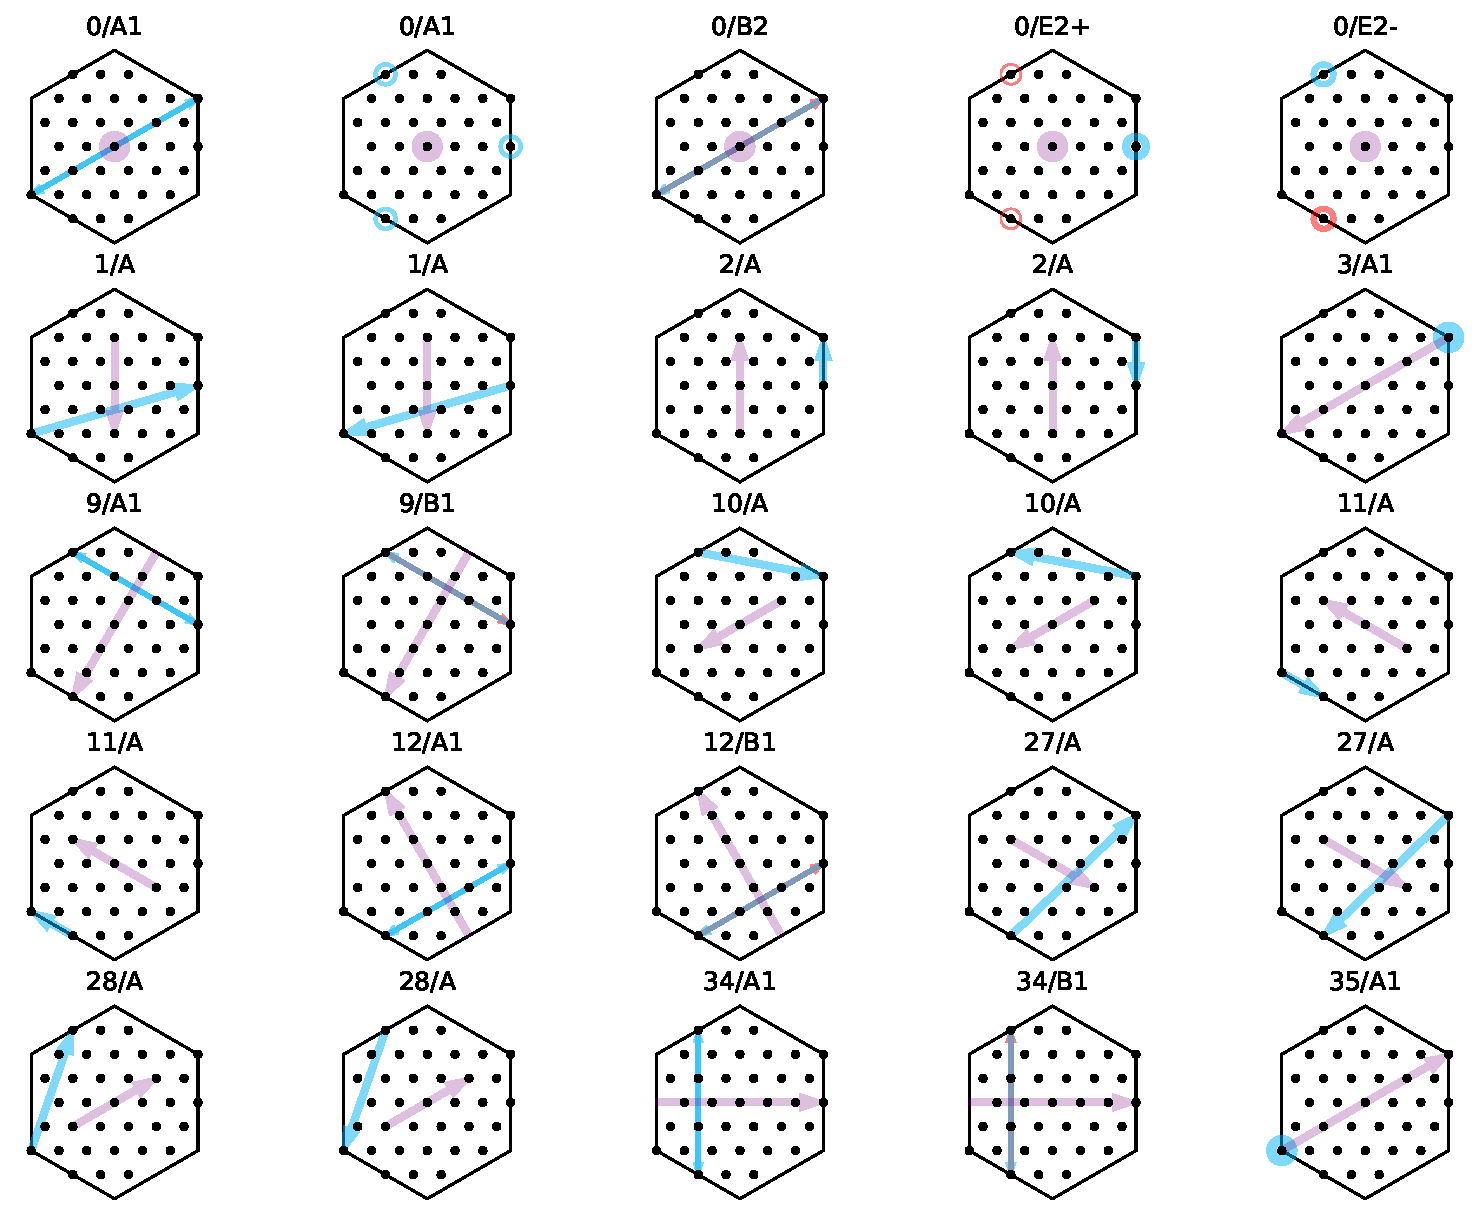
\includegraphics[width=\linewidth]{BZ_KM.pdf}}
    \caption{Example of different momentum shells with their irreducible representations. The number on the left side of "/" in the titles indicates the shell, and on the right side is the irreducible representations of the little group. The head of the pink arrow shows the total momentum $P$; the tail shows $-P$. Only at zero momentum there is a circle. Blue/Red arrows point the relative momentum. The color indicates the phase of the operators (red = $\pi$, blue = 0) and the relative thickness indicates the relative weight of that state.}
    \label{fig:mom_shells}
\end{figure}
We construct total momenta shells with different relative momentum in each one. The transformation of the operators is represented by the little group of $\mathcal{G}$ which preserves the total momentum $\vec{P}$. We can find the irreducible representations for each momentum shell (example in \cref{fig:mom_shells}). The momentum labeling of the correlation functions can therefore be changed to
\begin{equation}
  \vec{k},\vec{s} \longrightarrow \vec{P},\vec{p},\rho;
\end{equation}
where $\vec{P} = \vec{k}+\vec{s}$ is the total momentum, $\vec{p} = \frac{\vec{k}-\vec{s}}{2}$ is the relative momentum, and $\rho$ is an irreducible representation of the little group~\cite{evan}.